\documentclass[border=2pt]{standalone}
\usepackage{tikz}
\usetikzlibrary{arrows.meta, positioning, fit, backgrounds, shapes.geometric}

\definecolor{orxblue}{HTML}{0072B2}
\definecolor{orxorange}{HTML}{E69F00}

\tikzset{
  orx/.style={
    font=\sffamily\footnotesize,
    >={Stealth[round, length=4pt, width=3pt]},
    line width=0.5pt,
    node distance=4mm and 9mm,
  },
  block/.style={
    draw=black!55, fill=white, rounded corners=1pt,
    minimum height=7mm, minimum width=35mm, inner sep=3pt, align=center,
  },
  ours/.style={
    block, draw=orxblue, fill=orxblue!7, line width=0.7pt,
    minimum width=49mm,
  },
  muted/.style={
    block, draw=black!30, fill=black!3, text=black!70,
    minimum width=43mm,
  },
  data/.style={
    draw=black!45, fill=black!4, trapezium, trapezium left angle=72,
    trapezium right angle=108, trapezium stretches body,
    minimum height=7mm, minimum width=44mm, inner sep=3pt, align=center,
  },
  flow/.style={->, draw=black!65},
  backflow/.style={->, draw=orxorange, dashed},
  edgelbl/.style={
    font=\sffamily\scriptsize, text=black!60, inner sep=1.5pt, fill=white,
  },
  stage/.style={
    draw=black!25, dashed, rounded corners=2pt, inner sep=5pt,
    minimum width=180mm,
  },
  stagelbl/.style={font=\sffamily\scriptsize\itshape, text=black!55},
}

\begin{document}
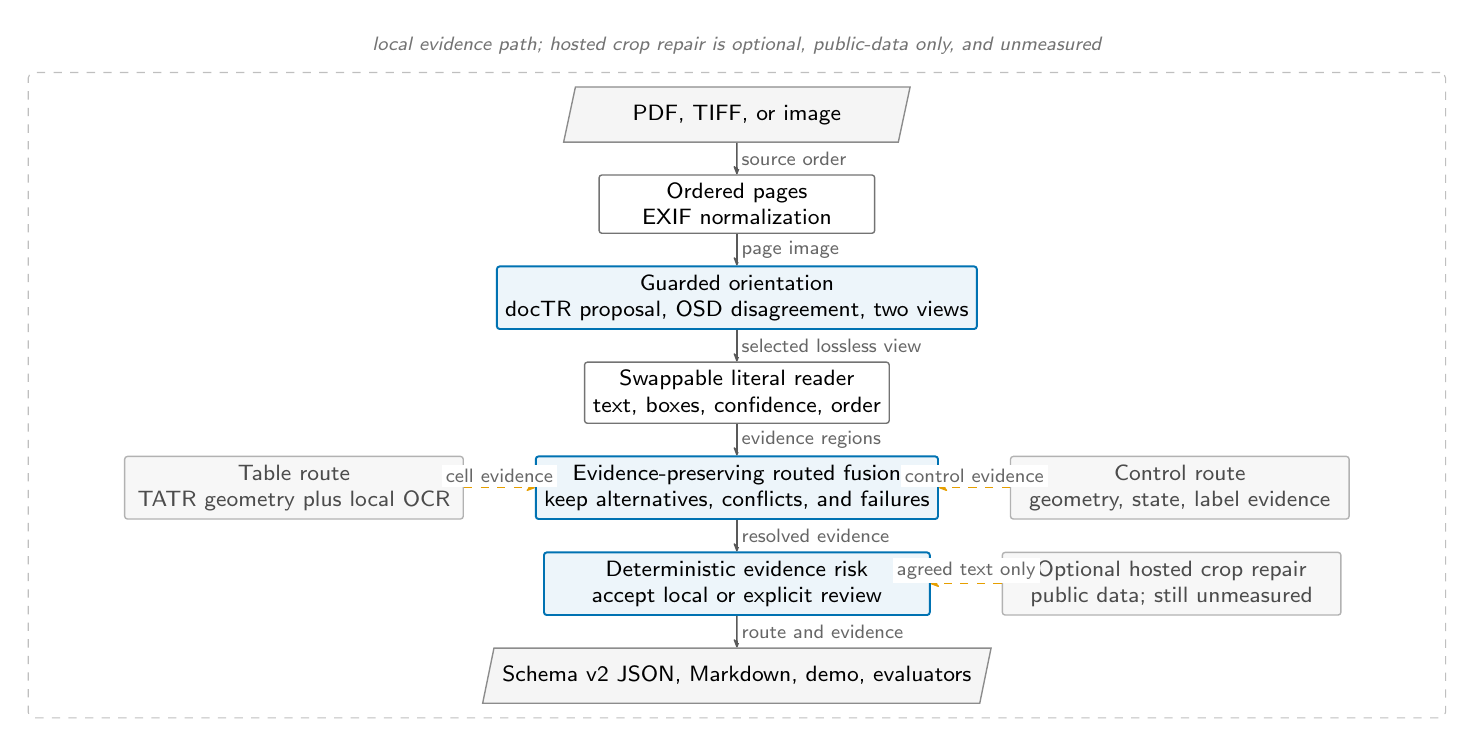
\begin{tikzpicture}[orx]
  \node[data] (input) {PDF, TIFF, or image};
  \node[block, below=of input] (pages) {Ordered pages\\EXIF normalization};
  \node[ours, below=of pages] (orientation) {Guarded orientation\\docTR proposal, OSD disagreement, two views};
  \node[block, below=of orientation] (reader) {Swappable literal reader\\text, boxes, confidence, order};
  \node[ours, below=of reader] (fusion) {Evidence-preserving routed fusion\\keep alternatives, conflicts, and failures};
  \node[ours, below=of fusion] (risk) {Deterministic evidence risk\\accept local or explicit review};
  \node[data, below=of risk] (output) {Schema v2 JSON, Markdown, demo, evaluators};

  \node[muted, left=of fusion] (tables) {Table route\\TATR geometry plus local OCR};
  \node[muted, right=of fusion] (controls) {Control route\\geometry, state, label evidence};
  \node[muted, right=of risk] (repair) {Optional hosted crop repair\\public data; still unmeasured};

  \draw[flow] (input) -- node[edgelbl, right] {source order} (pages);
  \draw[flow] (pages) -- node[edgelbl, right] {page image} (orientation);
  \draw[flow] (orientation) -- node[edgelbl, right] {selected lossless view} (reader);
  \draw[flow] (reader) -- node[edgelbl, right] {evidence regions} (fusion);
  \draw[flow] (fusion) -- node[edgelbl, right] {resolved evidence} (risk);
  \draw[flow] (risk) -- node[edgelbl, right] {route and evidence} (output);
  \draw[backflow] (tables) -- node[edgelbl, above] {cell evidence} (fusion);
  \draw[backflow] (controls) -- node[edgelbl, above] {control evidence} (fusion);
  \draw[backflow] (repair) -- node[edgelbl, above] {agreed text only} (risk);

  \begin{scope}[on background layer]
    \node[stage, fit=(input)(pages)(orientation)(reader)(fusion)(risk)(output)(tables)(controls)(repair)] (local) {};
  \end{scope}
  \node[stagelbl, above=1mm of local] {local evidence path; hosted crop repair is optional, public-data only, and unmeasured};
\end{tikzpicture}
\end{document}
